\documentclass[UTF8]{ctexart}
\usepackage{amsmath}
\usepackage{float}
\usepackage{indentfirst}
\usepackage{listings}
\usepackage{xcolor}
\lstset{
    %backgroundcolor=\color{red!50!green!50!blue!50},%代码块背景色为浅灰色
    rulesepcolor= \color{gray}, %代码块边框颜色
    breaklines=true,  %代码过长则换行
    numbers=left, %行号在左侧显示
    numberstyle= \small,%行号字体
    %keywordstyle= \color{red},%关键字颜色
    %commentstyle=\color{green!90}, %注释颜色
    frame=shadowbox%用方框框住代码块
    }
\usepackage{graphicx}
\usepackage[a4paper, left = 3.17cm, right = 3.17cm, top=2.54cm, bottom=2.54cm]{geometry}
\setlength{\parindent}{2em}
\title{第六讲-习题}
\author{姜帆}
\date{\today}
\begin{document}
\maketitle
\tableofcontents
\newpage
\section{证明题}
\indent 寻找最小二乘解:
\begin{equation}
{min}_y = \left\|Dy\right\|_2^2  \qquad s.t.\left\|y\right\|=1
\end{equation}
\indent 对$D^TD$做SVD分解得到下式:
\begin{equation}
D^TD = \sum_{i=1}^4\sigma^2_iu_iu_j^T
\end{equation}
\indent 其中$\sigma^2$为$D^TD$的奇异值,$u_i$为$D^TD$的奇异向量。$D^TD$为对称矩阵,因此奇异值分解与特征值分解得到的结果相同。
根据SVD分解推导证明过程可以知道,对$D$进行SVD分解,奇异值为对$D^TD$做特征值分解得到的特征值的平方根,特征向量$V$为右奇异向量,
其中大于$k=rank(D)$维度的分量都在$D$的零空间中,即$AV_i=0(i>k)$,也就是说$u_4$是$Ay=0$的解。\\
\indent 当取$y=u_4$时,即取奇异值$\sigma^2_4$最小对应的奇异向量作为最小二乘的解,此时有:
\begin{equation}
\begin{aligned}
& \left\|Dy\right\|_2^2 \\
&=y^TD^TDy\\
&=u_4^TD^TDu_4\\
&=\sigma^2_4u_4^Tu_4\\
&=\sigma^2_4
\end{aligned}
\end{equation}
\indent 此时目标函数取得最小。因此$y=u_4$为${min}_y = \left\|Dy\right\|_2^2 $的解。\\
\newpage
\section{代码实践题}
\indent 对$D^TD$做$SVD$分解,提取奇异值最小对应的奇异向量(由于$D^TD$为对称矩阵,左右奇异向量相同,且对$D^TD$做特征值分解得到的特征值、
特征向量和做奇异值分解得到的奇异值和奇异向量相同)即为最小二乘的解,约掉第四维后便得到路标点的坐标。\\
\begin{figure}[H]
\centering
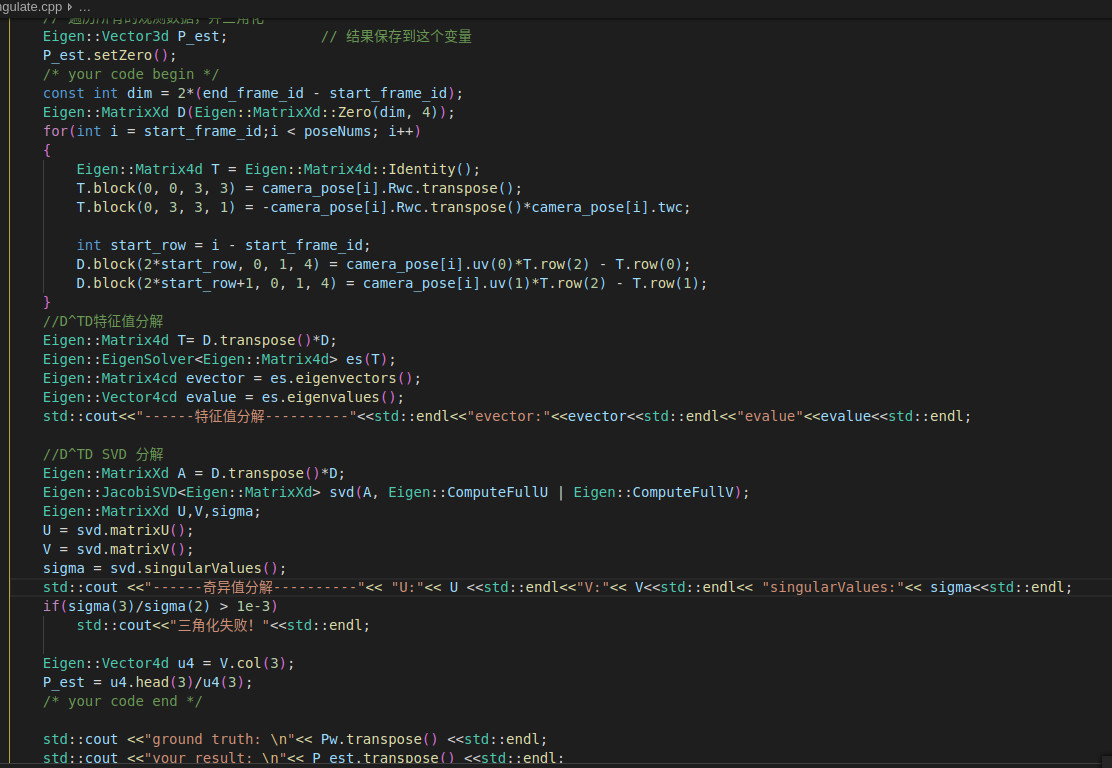
\includegraphics[width=0.8\textwidth]{1.1.jpg}    
\caption{代码补充}
\label{img0}
\end{figure}
\indent  对$D^TD$做特征值分解以及做奇异值分解结果,可以看出奇异值与特征值,奇异向量与特征向量相等:
\begin{figure}[H]
\centering
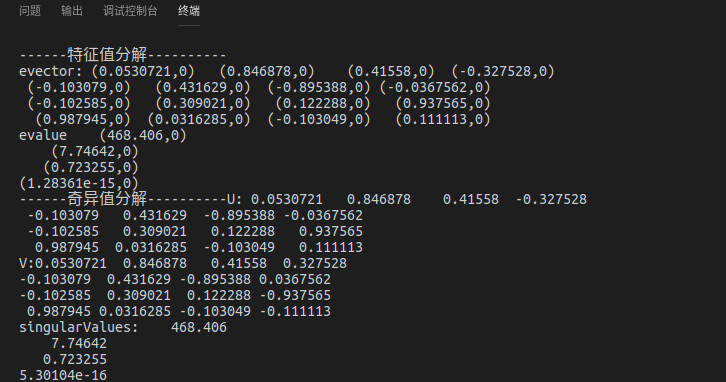
\includegraphics[width=0.8\textwidth]{1.2.jpg}    
\caption{特征值分解和奇异值分解结果}
\label{img0}
\end{figure}
\begin{figure}[H]
\centering
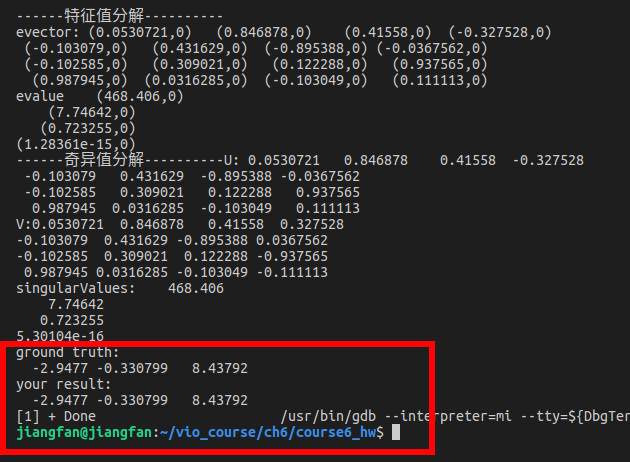
\includegraphics[width=0.8\textwidth]{1.3.jpg}    
\caption{路标点坐标计算结果}
\label{img0}
\end{figure}
\end{document}